% Source: https://tex.stackexchange.com/a/681629/6880
 
\documentclass{article}
\usepackage{tikz}

\begin{document}

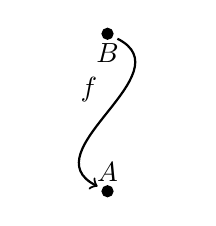
\begin{tikzpicture}[scale=2,rotate=90]   
  \draw[thick, ->, shorten <= 4pt, shorten >= 4pt] 
    (0.5,0) .. controls (0.25,-0.5) 
    and 
    (-0.25,0.5) .. (-0.5,0) 
    node[pos=0.5, above left] {$f$}; 
  \filldraw[black]
    (-0.5,0) circle (1pt) node[above] {$A$};   
  \filldraw[black] (0.5,0)
    circle (1pt) node[below] {$B$};
\end{tikzpicture}

\end{document}